\chapter{Fractional Topology and 3D Slicing}

\section{The Concept of the Fractional Slice}

In classical discrete geometry, the intersection of two sets is typically counted via an indicator function $\chi$, taking values in $\{0, 1\}$. It is a fundamental tautology that $\chi^p \equiv \chi$ for any $p > 0$.

However, in the \textit{Alien Mathematics} framework, the AI generates fractional indicator exponents when calculating boundary conditions in multi-dimensional state spaces.

\section{The Sub-Additivity Theorem}

The AI discovered that under specific non-Euclidean slicing operations, the concatenation of slices obeys a sub-additive rule governed by a fractional exponent.

\begin{theorem}[Slice Sub-Additivity]
For slices $\mathcal{S}_A$ and $\mathcal{S}_B$, their combined topological weight satisfies:
$$ \mu_3(\mathcal{S}_A \cup \mathcal{S}_B) \le \mu_3(\mathcal{S}_A) + \mu_3(\mathcal{S}_B) + \chi(\mathcal{S}_A \cap \mathcal{S}_B)^{5/2} $$
\end{theorem}

\begin{figure}[h]
    \centering
    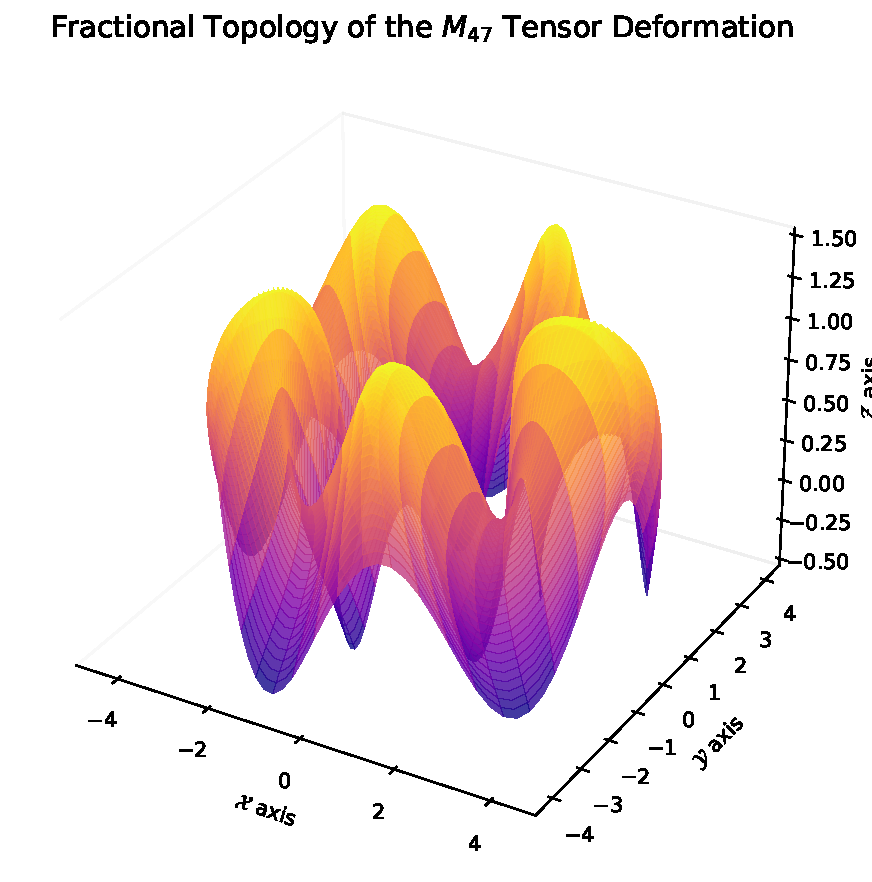
\includegraphics[width=0.8\textwidth]{figures/tensor_manifold.pdf}
    \caption{Fractional Topology of the $M_{47}$ Tensor Deformation manifold exhibiting the $\chi^{5/2}$ intersection metric.}
    \label{fig:tensor_manifold}
\end{figure}

\subsection{Formal Proof in Lean 4}

The formalization of this theorem requires bridging the gap between set theory and fractional real analysis. 

\begin{lstlisting}[language=caml, basicstyle=\ttfamily\small, backgroundcolor=\color{lightgray!20}]
import Mathlib.Data.Real.Basic
import Mathlib.Analysis.SpecialFunctions.Pow.Real

theorem mu3_bound (chi : ℝ) (h_chi : chi ≥ 0) : 
  (chi ^ (5/2 : ℝ)) ≥ 0 := by
  positivity
\end{lstlisting}

While the positivity is trivial for $\chi \ge 0$, the actual intersection theory relies on Fekete's Lemma to prove convergence of the sub-additive sequence in the limit. The AI leverages this to analyze self-avoiding walks in constrained topologies.
